% Created 2020-05-26 Tue 22:48
% Intended LaTeX compiler: pdflatex
\documentclass[presentation]{beamer}
\usepackage[utf8]{inputenc}
\usepackage[T1]{fontenc}
\usepackage{graphicx}
\usepackage{grffile}
\usepackage{longtable}
\usepackage{wrapfig}
\usepackage{rotating}
\usepackage[normalem]{ulem}
\usepackage{amsmath}
\usepackage{textcomp}
\usepackage{amssymb}
\usepackage{capt-of}
\usepackage{hyperref}
\usetheme{default}
\author{Rebecca Skinner}
\date{\today}
\title{An Introduction To Networking}
\hypersetup{
 pdfauthor={Rebecca Skinner},
 pdftitle={An Introduction To Networking},
 pdfkeywords={},
 pdfsubject={},
 pdfcreator={Emacs 26.3 (Org mode 9.3.6)},
 pdflang={English}}
\begin{document}

\maketitle
\begin{frame}{Outline}
\tableofcontents
\end{frame}


\begin{frame}[label={sec:org6e32325}]{An Introduction to Networking}
\pause
\begin{itemize}
\item Twitter: \href{https://twitter.com/cercerilla/}{@cercerilla}
\end{itemize}
\pause
\begin{itemize}
\item Github: \url{https://github.com/rebeccaskinner}
\end{itemize}
\pause
\begin{itemize}
\item \url{https://github.com/rebeccaskinner/presentations}
\end{itemize}
\pause
\begin{itemize}
\item License \href{https://creativecommons.org/licenses/by-sa/4.0/}{CC BY-SA 4.0}
\item All views are my own and don't represent the views of my employer
\end{itemize}
\end{frame}

\begin{frame}[label={sec:orgde6d4f5}]{The Internets}
\begin{center}
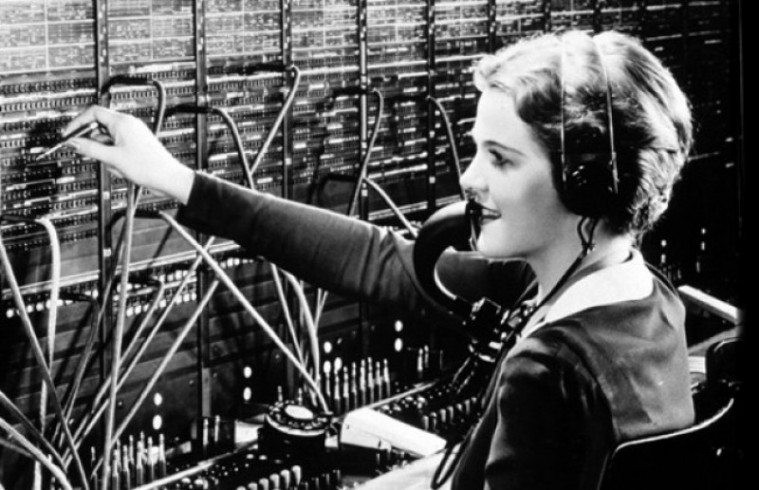
\includegraphics[width=.9\linewidth]{./switch-operator.jpeg}
\end{center}
\end{frame}

\begin{frame}[label={sec:org0e92236}]{Who Is This Talk For?}
If you work with software that depends on communication between two or
more computers, it's helpful for you to know a bit about how
networking works.
\end{frame}

\begin{frame}[label={sec:org63470c6}]{Networks are Invisible and Ubiquitious}
The growth of the web is the most obvious way that networks have
become a ubiquitious part of the growth of networking, but there are
other areas where networking has become pervasive:

\begin{itemize}
\item Distributed Compute
\item IoT
\item Mobile
\item Web
\item Multimedia / Streaming
\end{itemize}
\end{frame}

\begin{frame}[label={sec:orgb7ba256}]{Networks are Poorly Understood}
\begin{center}

\includegraphics[width=.9\linewidth]{./no-idea-what-im-doing-dog.png}
\end{center}
\end{frame}

\begin{frame}[label={sec:org76269e3}]{A Browser Walks Into An Address Bar And Says}
\begin{center}
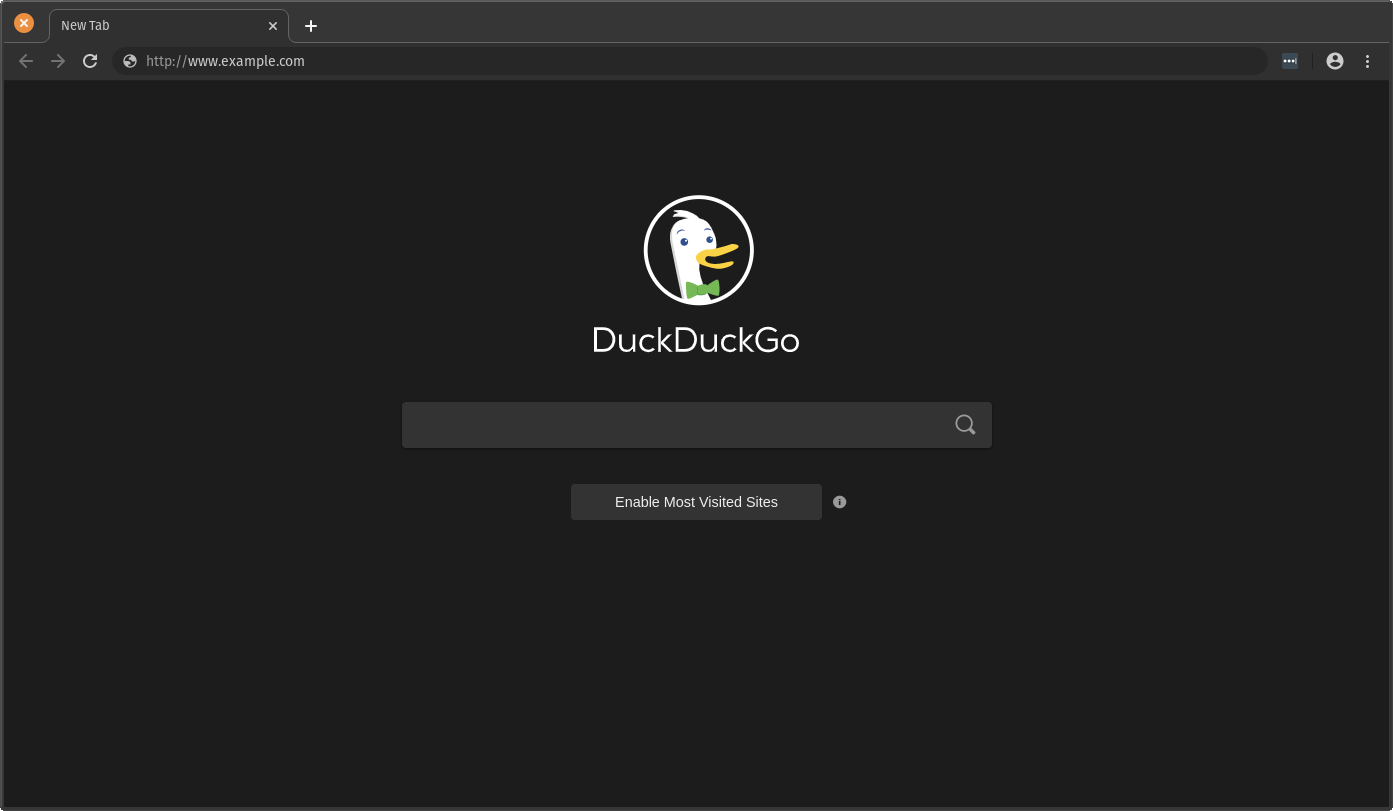
\includegraphics[width=.9\linewidth]{./browser-example-com.png}
\end{center}
\end{frame}

\begin{frame}[label={sec:org2e25571}]{A Browser Walks Into An Address Bar And Says}
\begin{itemize}
\item Browser
\end{itemize}
\pause
\begin{itemize}
\item HTTP Request \& Response
\end{itemize}
\pause
\begin{itemize}
\item DNS Lookup
\end{itemize}
\pause
\begin{itemize}
\item TCP Handshake
\end{itemize}
\pause
\begin{itemize}
\item IP Routing
\end{itemize}
\pause
\begin{itemize}
\item Ethernet Switching
\end{itemize}
\pause
\begin{itemize}
\item Runtime Socket Code
\end{itemize}
\pause
\begin{itemize}
\item Kernel Networking Code
\end{itemize}
\pause
\begin{itemize}
\item NIC Device Driver Code
\end{itemize}
\pause
\begin{itemize}
\item PCI, DMA, \ldots{}
\end{itemize}
\pause
\begin{itemize}
\item CAT5\ldots{}
\end{itemize}
\end{frame}

\begin{frame}[label={sec:orgcfcbd78}]{The Seven Layer Burrito}
\begin{center}
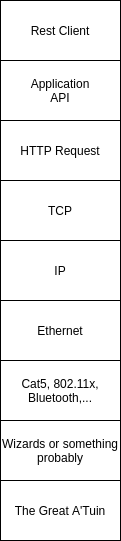
\includegraphics[height=0.8\textheight]{./osi-model-extended.png}
\end{center}
\end{frame}

\begin{frame}[label={sec:org9c121c6}]{The OSI and TCP/IP Models}
\begin{itemize}
\item The "Seven Layer" OSI model defines a somewhat idealized stratification of network protocls
\item The TCP/IP focuses more on encapsulation and acknowledges the fuzziness of the real-world
\end{itemize}
\end{frame}

\begin{frame}[label={sec:orgb7e5b3a}]{The OSI Model}
The OSI Model in its natural habitat

\begin{center}
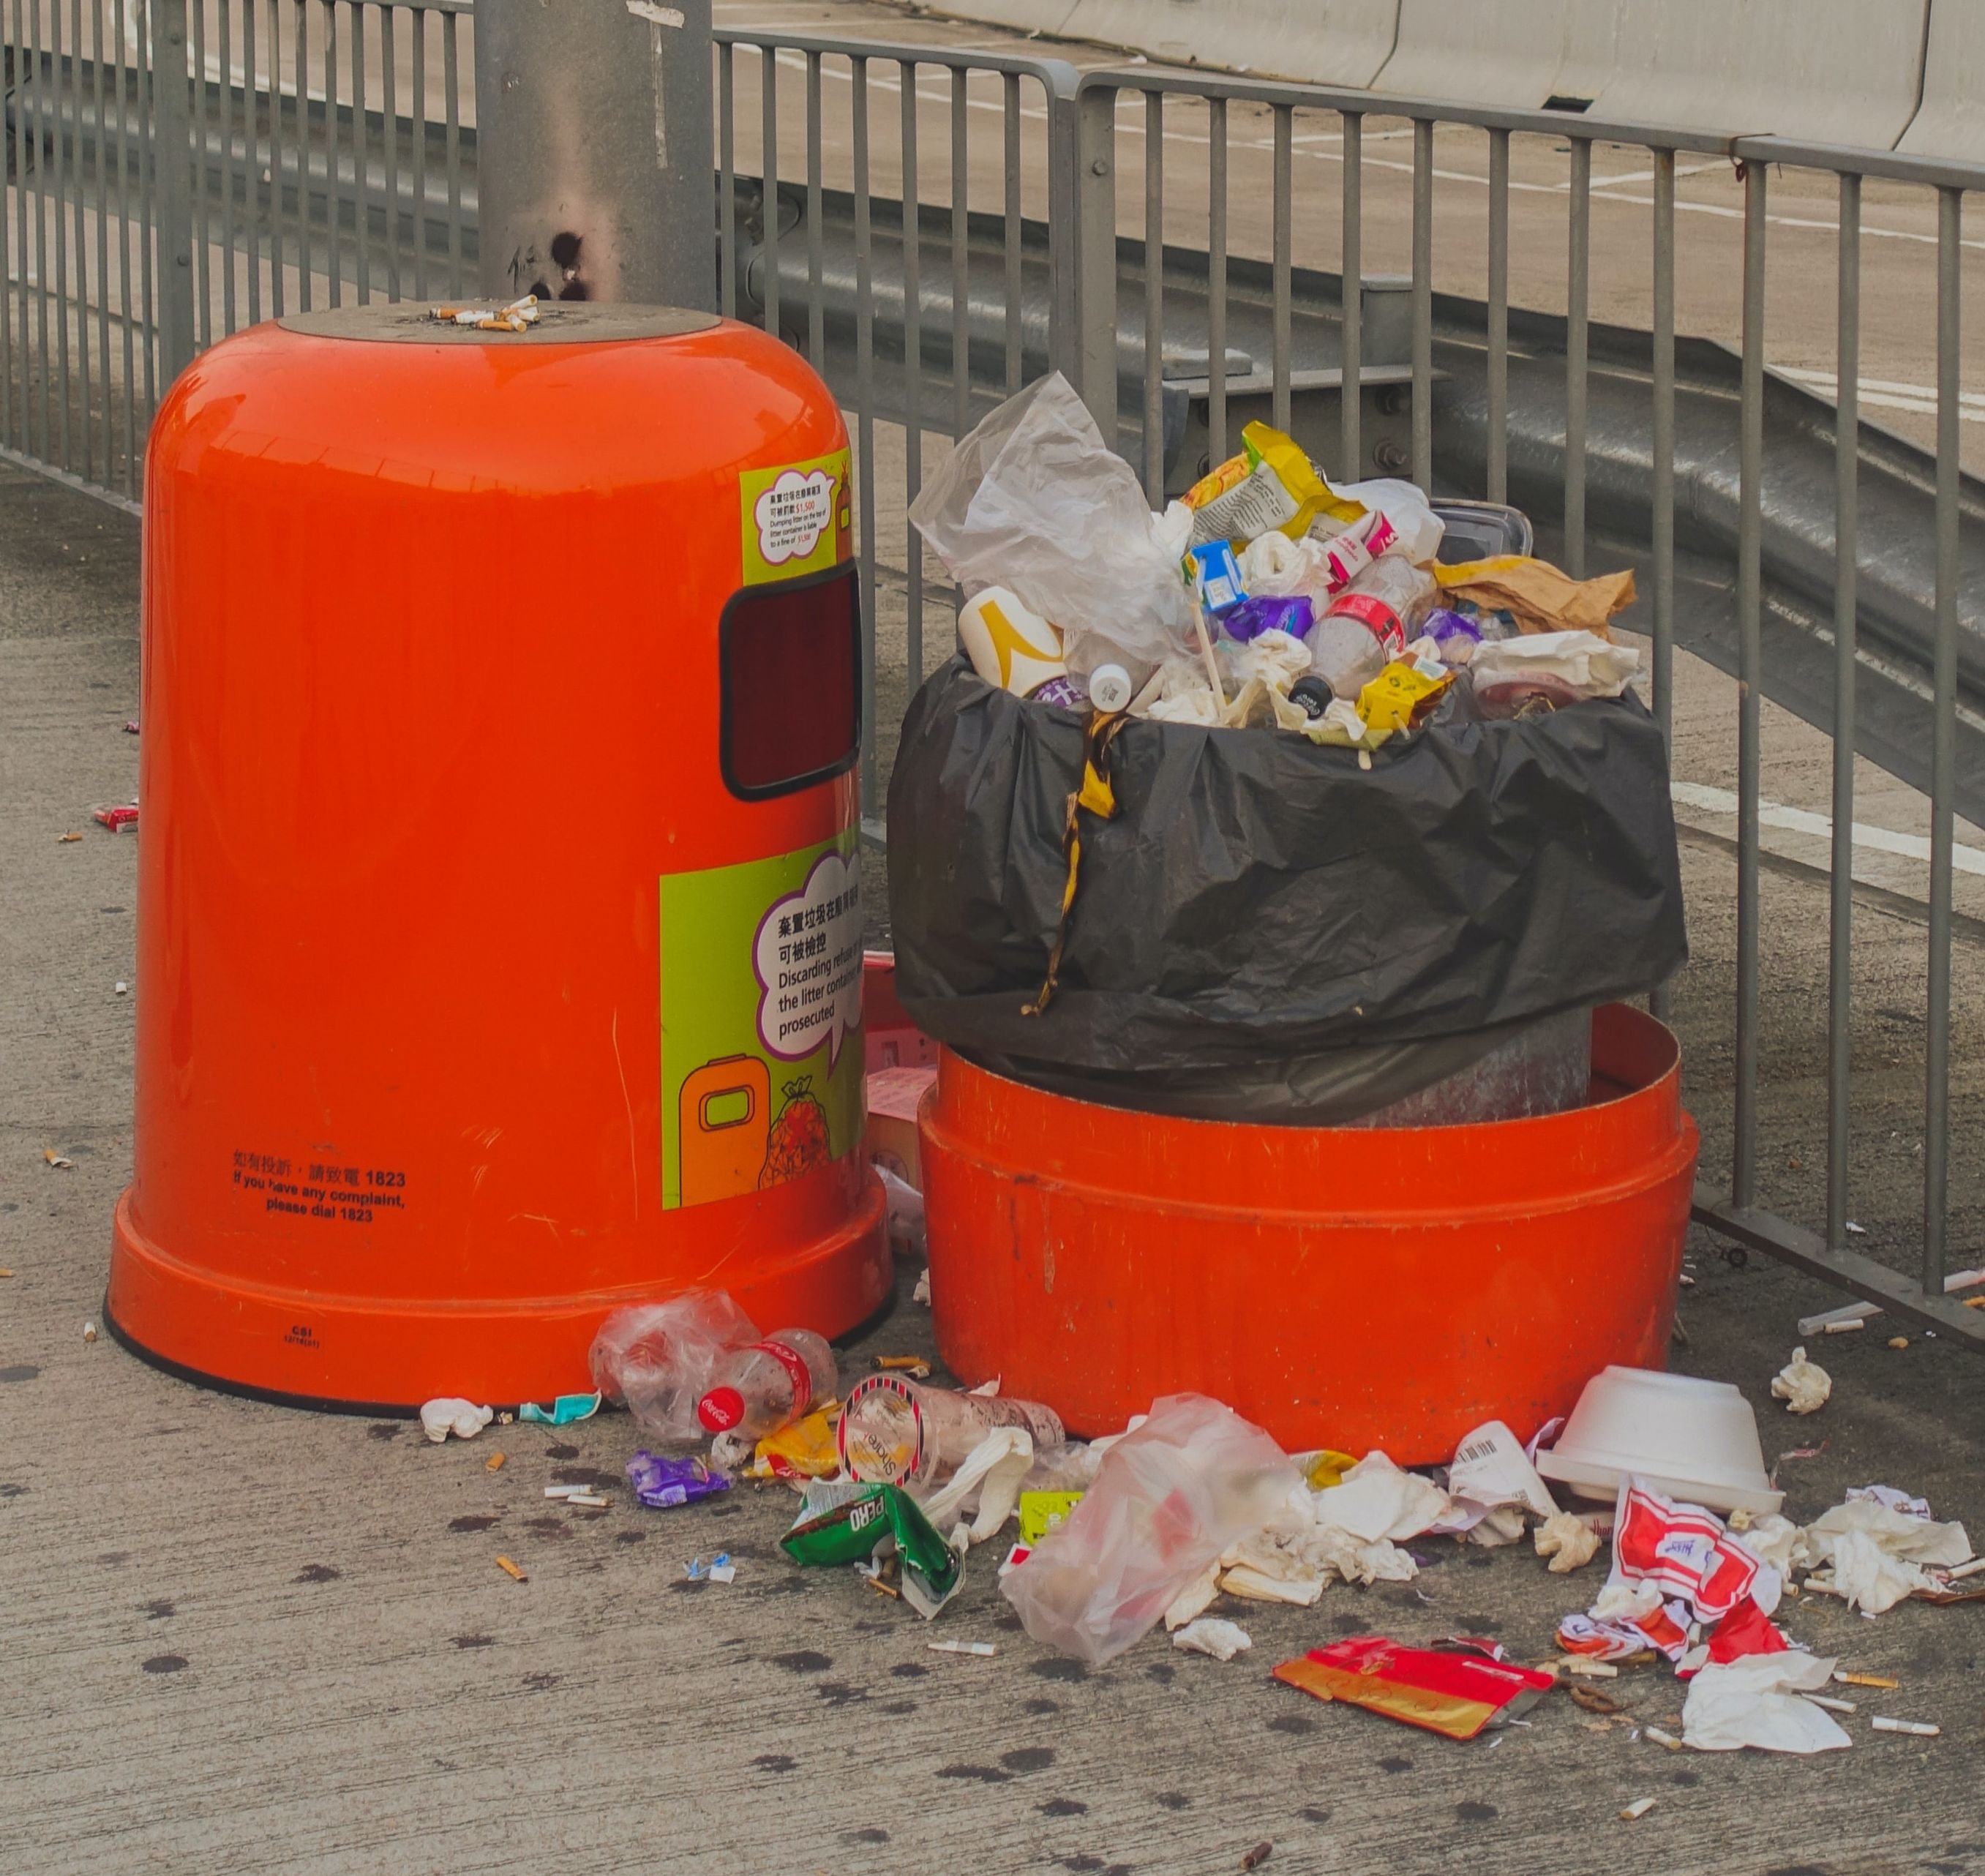
\includegraphics[height=0.8\textheight]{./garbage.jpg}
\end{center}
\end{frame}

\begin{frame}[label={sec:org2366317}]{Where Do We Go From Here?}
\begin{itemize}
\item DNS
\item TCP
\item IP
\item Routing
\item Switching
\end{itemize}
\end{frame}

\begin{frame}[label={sec:orgb3c6200}]{DNS}
What is DNS?
\pause
DNS is basically how we translate between a domain name, like
example.com, and an IP address, like 172.24.18.197.
\end{frame}

\begin{frame}[label={sec:org34ba428}]{AAAA++++ Would Look Up Again}
A DNS server has many different kinds of records that it can
serve. The details differ, but the ultimate goal is to provide
information about how to get data to some domain through the internet.

\pause
Some popular records include

\begin{itemize}
\item A
\item AAAA
\item CNAME
\item TXT
\item Abbey Road
\end{itemize}
\end{frame}

\begin{frame}[label={sec:org2be301a}]{Imminent Domain}
Not every DNS server knows about every domain in the world.  DNS is
hierarchical. A DNS lookup is like that book "Are you my mother?"
except at the end of the book there's like an 80\% chance your mother
was randomly generated in order to serve you a tracking pixel.

\pause
\begin{itemize}
\item Authoritative Servers
\item Recursive Servers
\end{itemize}
\end{frame}

\begin{frame}[label={sec:org3b30494}]{Untitled}
\begin{center}
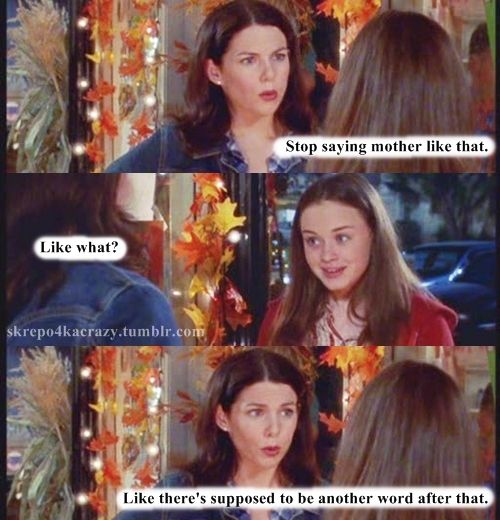
\includegraphics[height=0.8\textheight]{./gg.jpg}
\end{center}
\end{frame}

\begin{frame}[label={sec:org971ddb3}]{TCP, UDP, We All P for IP\ldots{} or Something?}
IP is how your data gets around the internet. TCP and UDP are how your
data gets around the internet with more letters.
\end{frame}

\begin{frame}[label={sec:org2c5ff37}]{Ports}
TCP and UDP let you multiplex streams of data over a single IP link
using ports. IANA has a list of common common ports that people used
to use before they just started tunneling everything over 443 because
corporate firewalls are a joke.
\end{frame}

\begin{frame}[label={sec:org92a3697}]{SYNACK Break}
Most traffic on the internet uses TCP.  TCP tries to guarantee that
packages arrive and are reassembled in the right order. TCP
connections start with the "three-way handshake" or the currently more
popular "three-way hand-wave from at least 6 feet away"
\end{frame}

\begin{frame}[label={sec:orgc988bae}]{Here's a really funny UDP joke}
I don't care if you get it

\pause
UDP works much faster because you don't even have to care if it
worked.
\end{frame}

\begin{frame}[label={sec:orgcb64cb8}]{IP}
TCP and UDP by themselves don't know how to go anywhere. IP is the
mechanism that allows data to get from one computer to another.  Well
kind of.  There are a bunch more slides still.
\end{frame}

\begin{frame}[label={sec:org1871bc3}]{Roto-Routers}
An IP address is like a PO box.

Routers are like electronic devices that use protocols like BGP to
efficiently generate compact representations of sparse mappings
between networks, allowing them hand off data payloads encapsulated
with IP headers from one device to another until it can be delivered
to the correct address.
\pause
Also they mangle packets and send them out of order or not at all
sometimes so that's fun.
\end{frame}

\begin{frame}[label={sec:orgb0760c1}]{Put Them Somewhere Else}
\begin{center}
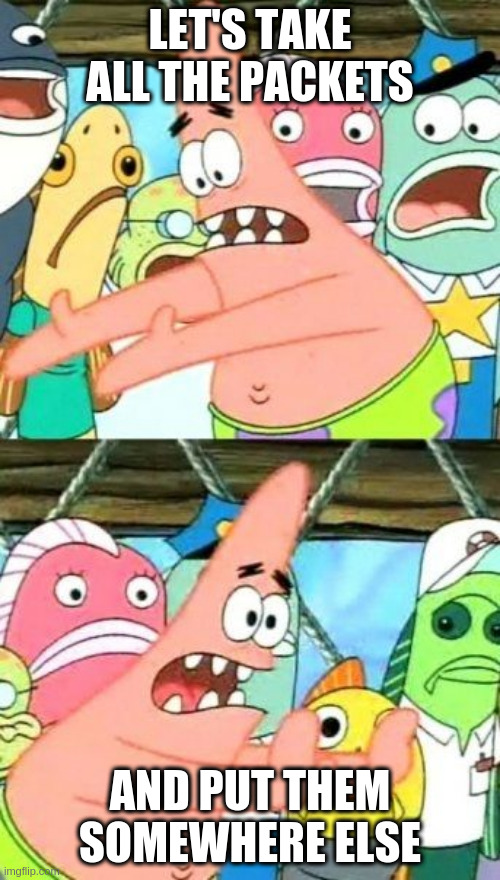
\includegraphics[height=0.8\textheight]{./somewhere-else.jpg}
\end{center}
\end{frame}

\begin{frame}[label={sec:org55247f7}]{Subnets}
Not everything needs to get routed across the internet.  Subnets
define the local part of your network. They can be written using
netmask notation (255.0.0.0) or CIDR notation (/8).
\end{frame}

\begin{frame}[label={sec:org9efa657}]{Switching}
\begin{center}
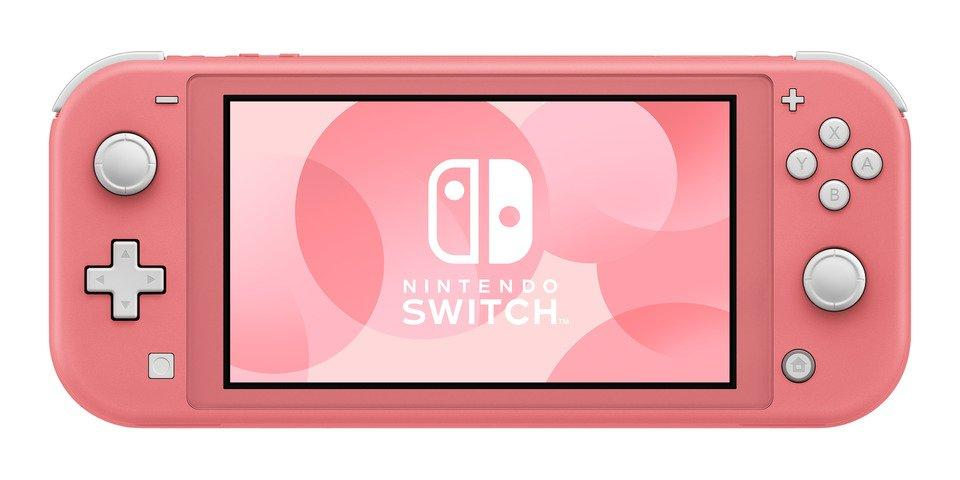
\includegraphics[width=.9\linewidth]{./switch.jpeg}
\end{center}
\end{frame}

\begin{frame}[label={sec:org92ea1e3}]{The Luminiferous Æthernet}
Within a local network, switching is responsible for delivering
packets from one computer to another. You can think of your home
switch like a roundabout: Nobody knows how to use them but at least
they are cheap.
\end{frame}

\begin{frame}[label={sec:orgde33ffe}]{Whadda Ya Have, Mac?}
MAC addresses are how different devices on the same switch can talk to
one another and how you can get free hotel wifi.
\end{frame}

\begin{frame}[label={sec:orge000fb3}]{ARP and other capital letters}
ARP tables are how devices on a switching network know how to get
messages back and forth to one another.
\end{frame}

\begin{frame}[label={sec:orgd414903}]{Gateways}
\begin{center}
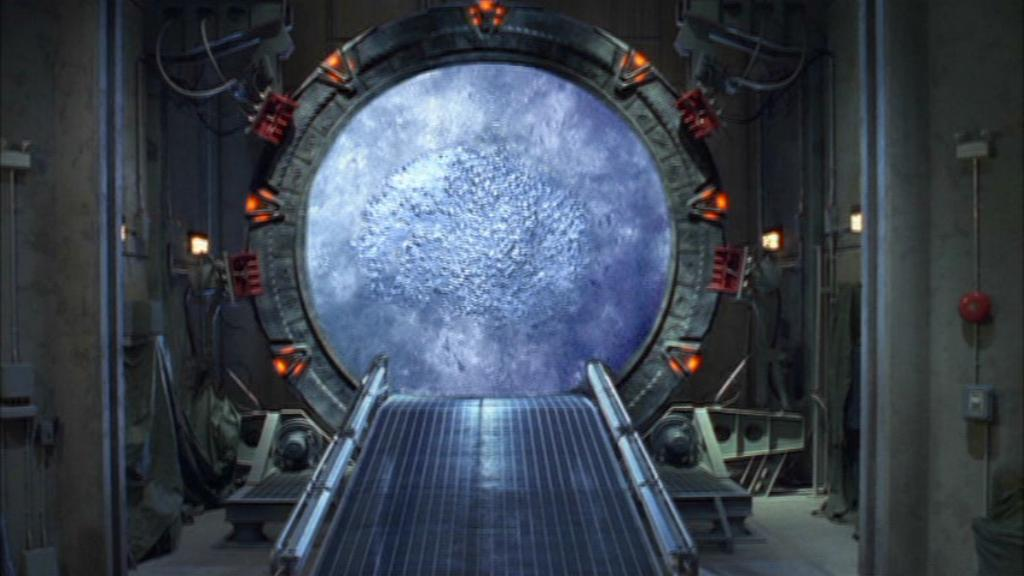
\includegraphics[width=.9\linewidth]{./stargate.jpg}
\end{center}
\end{frame}

\begin{frame}[label={sec:orgc7c52a5}]{DHCP and Local Routes}
DHCP is what's generally responsible for getting each physical network
device an IP address. It also pushes down information like where the
DNS servers are and what the default gateway is that you should use.
\end{frame}

\begin{frame}[label={sec:org4e66a70}]{Statement?}
Aggressively made, but with the approximate structure of a question?
\end{frame}
\end{document}